\documentclass{article}
\usepackage{graphicx,amsmath,latexsym}
\usepackage{color,psfrag,boxedminipage,amssymb}
%\usepackage[latin1]{inputenc}
%\usepackage[swedish]{babel}
%\usepackage{draftcopy}
\usepackage{tikz}
\usepackage{pgf}
\usetikzlibrary{positioning,arrows}

\newcommand{\st}{\ensuremath{\boldsymbol{s}_k(\boldsymbol{\theta})}}
\newcommand{\St}{{\mathbf S}\ensuremath{(\boldsymbol{\theta})}}
\newcommand{\phibf}{\ensuremath{\boldsymbol{\phi}}}
\newcommand{\varphibf}{\ensuremath{\boldsymbol{\varphi}}}
\def \phibfh{\ensuremath{\hat{\boldsymbol{\phi}}}}
\renewcommand{\sp}{\ensuremath{\boldsymbol{s}(\boldsymbol{\phi})}}
\newcommand{\hp}{\ensuremath{\boldsymbol{h}(\boldsymbol{\phi})}}
\newcommand{\thk}{\ensuremath{\boldsymbol{\theta}_k}}
\renewcommand{\th}{\ensuremath{\boldsymbol{\theta}}}
\newcommand{\alp}{\ensuremath{\boldsymbol{\alpha}}}
\def \thh{\ensuremath{\hat{\boldsymbol{\theta}}}}
\def \epsbf{\ensuremath{\boldsymbol{\epsilon}}}
\def \tht{\tilde{\th}}
\newcommand{\mubf}{\ensuremath{\boldsymbol{\mu}}}

\newcommand{\ctft}{\buildrel{{\cal F}}\over{\longleftrightarrow}}
\newcommand{\defin}{\buildrel{\triangle}\over{=}}

\def \Em{{\mathbb{E}}}



\def \abf{{\mathbf a}}
\def \Abf{{\mathbf A}}
\def \bbf{{\mathbf b}}
\def \Bbf{{\mathbf B}}
\def \cbf{{\mathbf C}}
\def \Cbf{{\mathbf C}}
\def \dbf{{\mathbf d}}
\def \Dbf{{\mathbf D}}
\def \ebf{{\mathbf e}}
\def \Ebf{{\mathbf E}}
\def \fbf{{\mathbf f}}
\def \Fbf{{\mathbf F}}
\def \gbf{{\mathbf g}}
\def \Gbf{{\mathbf G}}
\def \hbf{{\mathbf h}}
\def \Hbf{{\mathbf H}}
\def \ibf{{\mathbf i}}
\def \Ibf{{\mathbf I}}
\def \jbf{{\mathbf j}}
\def \Jbf{{\mathbf J}}
\def \kbf{{\mathbf k}}
\def \Kbf{{\mathbf K}}
\def \lbf{{\mathbf l}}
\def \Lbf{{\mathbf L}}
\def \mbf{{\mathbf m}}
\def \Mbf{{\mathbf M}}
\def \nbf{{\mathbf n}}
\def \Nbf{{\mathbf N}}
\def \obf{{\mathbf o}}
\def \Obf{{\mathbf O}}
\def \pbf{{\mathbf p}}
\def \Pbf{{\mathbf P}}
\def \qbf{{\mathbf q}}
\def \Qbf{{\mathbf Q}}
\def \rbf{{\mathbf r}}
\def \Rbf{{\mathbf R}}
\def \sbf{{\mathbf s}}
\def \Sbf{{\mathbf S}}
\def \tbf{{\mathbf t}}
\def \Tbf{{\mathbf T}}
\def \ubf{{\mathbf u}}
\def \Ubf{{\mathbf U}}
\def \vbf{{\mathbf v}}
\def \Vbf{{\mathbf V}}
\def \wbf{{\mathbf w}}
\def \Wbf{{\mathbf W}}
\def \xbf{{\mathbf x}}
\def \Xbf{{\mathbf X}}
\def \ybf{{\mathbf y}}
\def \Ybf{{\mathbf Y}}
\def \zbf{{\mathbf z}}
\def \Zbf{{\mathbf Z}}
\def \0bf{{\mathbf 0}}

\def \Emean{\mathbb{E}}

\def \Sibf{{\mathbf \Sigma}}
\def \xbbf{\mathbf{\bar{x}}}
\def \etr{\mbox{etr}}
\def \tr{\mbox{tr}}
\def \Tr{\mbox{Tr}}
\def \Cov{\mbox{Cov}}
\def \cost{\mbox{cost}}
\def \diag{\mbox{diag}}
\def \Lambf{{\mathbf{\Lambda}}}
\def \Gambf{{\mathbf{\Gamma}}}
\def \Sigbf{{\mathbf \Sigma}}
\newcommand{\rhobf}{\ensuremath{\boldsymbol{\rho}}}
\newcommand{\lambf}{\ensuremath{\boldsymbol{\lambda}}}
\newcommand{\nubf}{\ensuremath{\boldsymbol{\nu}}}

\newcounter{examplenr}[section]
\renewcommand{\theexamplenr}{\arabic{examplenr}}%{\thesection.\arabic{examplenr}}
\newenvironment{example}[1]{\vskip \baselineskip
\refstepcounter{examplenr}\noindent{{\bf
Example~\theexamplenr}\hskip .5em #1\\} }{\hrulefill $\Box$
 \vskip\baselineskip}



\newcounter{theoremnr}[section]
%\renewcommand{\thetheoremnr}{\thesection.\arabic{theoremnr}}
\renewcommand{\thetheoremnr}{\arabic{theoremnr}}
\newtheorem{A}[theoremnr]{Theorem}
\newcounter{theoremProofnr}[section]
%\renewcommand{\thetheoremProofnr}{\thesection.\arabic{theoremProofnr}}
\renewcommand{\thetheoremProofnr}{\arabic{theoremProofnr}}
\newtheorem{B}[theoremProofnr]{Proof of Theorem}
\newcounter{corollarynr}[section]
\renewcommand{\thecorollarynr}{\thesection.\arabic{corollarynr}}
\newtheorem{C}[corollarynr]{Corollary}
\newcounter{Lemmanr}[section]
\renewcommand{\theLemmanr}{\thesection.\arabic{Lemmanr}}
\newtheorem{D}[Lemmanr]{Lemma}
\newcounter{LemmaProofnr}[section]
\renewcommand{\theLemmaProofnr}{\thesection.\arabic{LemmaProofnr}}
\newtheorem{E}[LemmaProofnr]{Proof of Lemma}

\newcounter{propositionnr}[section]
\renewcommand{\thepropositionnr}{\arabic{propositionnr}}
\newtheorem{F}[propositionnr]{Proposition}
\newcounter{propositionProofnr}[section]
\renewcommand{\thepropositionProofnr}{\arabic{propositionProofnr}}
\newtheorem{G}[propositionProofnr]{Proof of proposition}

\newenvironment{working}{\color{blue}\sffamily\em}{}
\newenvironment{forslag}{\color{red}\sffamily\em}{}

\newcounter{definnr}[section]
\renewcommand{\thedefinnr}{\arabic{definnr}}
\newtheorem{J}[definnr]{Definition}



\usepackage{amsmath}
\usepackage{geometry}
\usepackage{caption}
\usepackage{lipsum} 
\geometry{a4paper}
\usepackage[backend=biber,style=ieee]{biblatex}
\usepackage{comment}
\bibliography{ref}
\begin{document}
\title{Solution for ML F16 assignment 2}
\author{Jonathan Hansen fdg890}
\maketitle

\section{K-Nearest Neighbors}
I have implemented the \textit{k}-nearest neighbor classifier in
\texttt{Python3}. I have made substantial use of the libraries \texttt{Pandas},
\texttt{Numpy} and \texttt{MatPlotLib}. All the code is gathered in a single
script called \texttt{irisknn.py}. Running it using "python3 irisknn.py" from
the terminal produces the requested plots and reports required values.

\subsubsection*{Question 1.1}
With my implementation i get the results presented below. Notice that the
training error for 1-NN is \(0\) as it should be. On the test data the
classifier performs equally well/bad with \textit{k}=\(1\) and \textit{k}=\(3\),
but the 5-NN performs substantially worse. This hints us that measuring size
only is maybe not a sufficient method for classifying iris', if we want to get
the error down below \(0.18\).

\begin{figure}[h]
\centering
\begin{tabular}{ |p{3cm}||p{3cm}|p{3cm}|p{3cm}|  }
 \hline
 \multicolumn{4}{|c|}{Training and testresults of \textit{k}-NN classifier
   for \textit{k} = 1,3,5}\\
 \hline
& \textit{k} = 1 & \textit{k} = 3 & \textit{k} = 5\\
 \hline
 Training error  & 0.0    & 0.14  & 0.17\\
 Test error      & 0.18  & 0.18  & 0.32\\
 \hline
\end{tabular}
\end{figure}

\subsubsection*{Question 1.2}
My cross-validation was done manually. I simply split the dataset into five
partitions and hard coded the fold. Since the data does not precide in any
particular order, this should not be a problem and it was the easiest way to
keep track of the rows. Figure \ref{fig:figure1} shows the averaged
cross-validation error as a function of the \textit{k} in the classifier. The
classifier performs best with \textit{k}=\(3\) why the results are reported in
the above table.

\begin{figure}[h]
  \centering
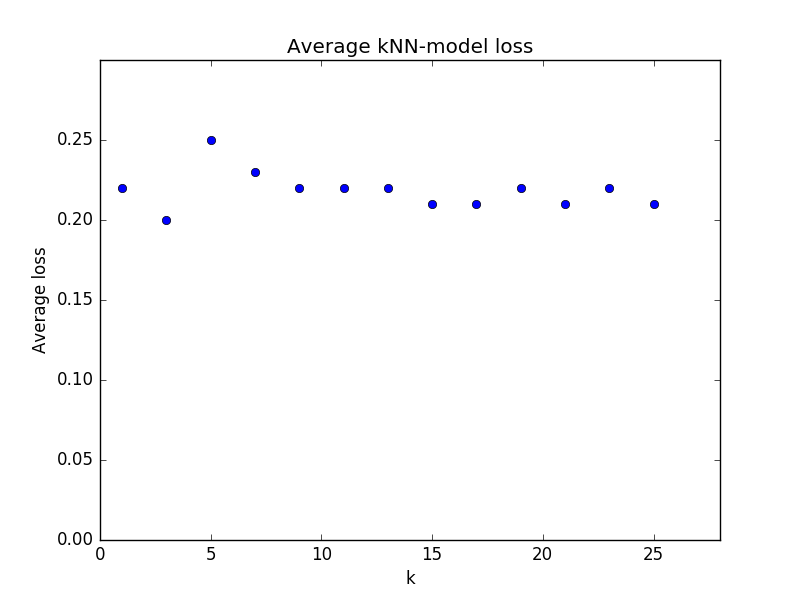
\includegraphics[scale=0.5]{figure_1}
\caption{Error as a function of \textit{k} in \text{k}-NN classifier}
\label{fig:figure1}
\end{figure}

\newpage
\subsubsection*{Question 1.3}
In the table below is the mean and variance of the input features and the mean
and variance after data normalization. The normalized data is supposed to be
zero-mean and it does come extremely close, but is not exactly zero. Variance is
1 as it should be. Using the affine linear mapping on the test data the sepal
width is significantly further from being zero-mean and unit length.

\begin{figure}[h]
\centering
\begin{tabular}{ |p{4cm}|p{1.5cm}|p{1.5cm}|p{1.5cm}|p{1.5cm}|  }
 \hline
 \multicolumn{5}{|c|}{Mean and variance of data before and after transformation}\\
 \hline
& Length mean & Width mean & Legth var & Width var \\
 \hline
 Training data              & 5.756 & 0.302 & 0.689 & 0.002 \\
 Transformed training data  & \(\approx\) 0  & \(\approx\) 0 & 1 & 1  \\
 Transformed test data      & 0.208 & 0.432 & 1.073 & 1.252 \\
 \hline
\end{tabular}
\end{figure}

In Figure \ref{fig:figure2} is shown the averaged cross-validation error as a
function of the \textit{k} in the classifier, this time run on the normalized
date. Compared to the previous plot you can see, that errors on an average are
lower, but also that they vary more. This time the classifier with
\textit{k}=\(11\) performs better.

\begin{figure}[h]
  \centering
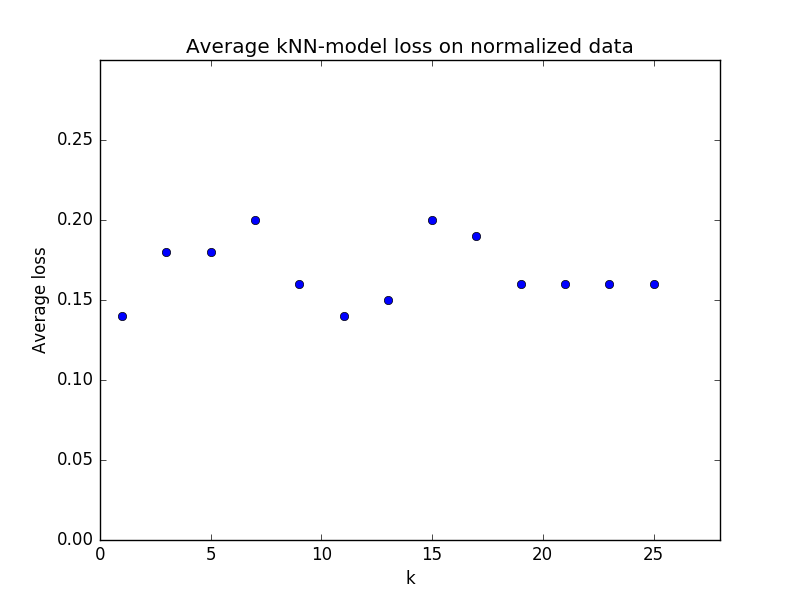
\includegraphics[scale=0.5]{figure_2}
\caption{Error as a function of \textit{k} in \text{k}-NN classifier on
  normalized data}
\label{fig:figure2}
\end{figure}
\newpage
Finally the table below shows the training and test error of the 11NN classifier
which the analysis pointed out as \textit{k}\(_{best}\). The table also shows
the result of the initial 3NN classification of the raw data for comparison. It
is interesting that 11NN classifier performs best, but only on training
transformed training data. However we should remember, that the transformation
of the test data was done with the affirm linear mapping that was found on the
training data. This hints us that there might be a tendency in test data that is
different than the training data. At the same time we have just two features to
perform our analysis on and just 100 training data points.

\begin{figure}[h]
\centering
\begin{tabular}{ |p{8cm}||p{2cm}|  }
 \hline
 \multicolumn{2}{|c|}{Error of initial 3NN and 11NN on normalized training
   and test data}\\
 \hline
& Error \\
 \hline
 3NN error, raw testdata       & 0.18  \\
 11NN train error, transformed data  & 0.14 \\
 11NN test error, transformed data & 0.26 \\ 
 \hline
\end{tabular}
\end{figure}



\newpage
\section{Markov’s inequality vs. Hoeffding’s inequality vs. binomial bound}
\subsubsection*{Question 2.1}
To bound the probability that \(\sum_{n=1}^{10} X_i\) we start by plugging
the given values into Markovs inequality:

\[
P\{S \ge 9\} \le \dfrac{\Em[S]}{9}
\]
\
Using the random variable we are given and linearity of expectation we get:

\[
P\{\displaystyle\sum_{n=1}^{10} X_i \ge 9\} \le \displaystyle\sum_{n=1}^{10}
\dfrac{\Em[X_i]}{9}
\]
\
\
Since we know that \(X_1\),...,\(X_{10}\) are i.i.d Bernoulli random variables
with bias \(\frac{1}{2}\) the expected value sums to \(\frac{5}{9}\). Thus we get:

\[
P\Big(\sum_{n=1}^{10} X_i \ge 9 \Big) \le \dfrac{5}{9}
\]

\subsubsection*{Question 2.2}
Focusing at first at the probability side of Hoeffding's inequeality we can use
the information given, and the result of the sum of expected valus from above,
to determine \(\varepsilon\):

\[
\mathbb{P}\left\{\displaystyle\sum_{n=1}^{10} X_i -
\Em\bigg[\displaystyle\sum_{n=1}^{10} X_i \bigg] \ge \varepsilon \right\} \Leftrightarrow
\mathbb{P}\left\{\displaystyle\sum_{n=1}^{10} X_i \ge \varepsilon + 5 \right\} \Rightarrow
\varepsilon = 4
\]
\
\
With this result we can find the bound we are asked for, since we know that
\(a_i=0\) and \(b_i=1\):

\[
P\Big(\sum_{n=1}^{10} X_i \ge 9 \Big) \le e^{-2(4)^2/\sum_{n=1}^{10}(1-0)^2} = e^{-\frac{16}{5}}
\]

\subsubsection*{Question 2.3}
We can use the normal binomial PMF to calculate the exact probability of the
event. For the sum of the 10 random variables to be equeal nine,
we need success on  9 of them since they are Bernoulli random
variables:

\[
P\Big(\sum_{n=1}^{10} X_i = 9 \Big) = {{10}\choose{9}} 0.5^9(1-0.5)^{10-9} \approx 0.0098
\]




\subsubsection*{Question 2.4}
Comparing the three results the most interesting thing to note is that
Hoeffdinger's inequality produces a much tighter bound than Markov's
inequality. From Markov's you can get the (mis)understanding that
\(\sum_{n=1}^{10} X_i \ge 9\) is a pretty likely event, which is not the
case. This inprecision could be much more dangorous in a sitaution where our
understanding of the distribution or expectations is a lot less intuitive than
it is in this case.



\section{The effect of scale (range) and normalization of random variables in Hoeffding’s inequality}
We begin by substituting \(\varepsilon\) with \(n\varepsilon\) in \texttt{Theorem 1.2}:

\[
\mathbb{P}\left\{\displaystyle\sum_{i=1}^{n} X_i -
\Em\bigg[\displaystyle\sum_{i=1}^{n} X_i \bigg] \ge n\varepsilon \right\}
\le e^{-2(n\varepsilon)^2/\sum_{i=1}^{n}(b_i-a_i)^2}
\]
\
\
Looking first at the righthand side of the inequality, in the corollary that
we have to prove \(X_i\) can only assume values 0 and 1, why we know that:

\[
\sum_{i=1}^{n}(b_i-a_i)^2 = n
\]
\
And therefor the entire righthand side of the inequality can be reduced to:

\[
e^{-2n\varepsilon^2}
\]
\
Looking at the lefthand side we can dividide by \(n\) on both
sides of the inequality giving us:

\[
\mathbb{P}\left\{\dfrac{1}{n}\displaystyle\sum_{i=1}^{n} X_i -
\dfrac{1}{n}\Em\bigg[\displaystyle\sum_{i=1}^{n} X_i \bigg] \ge \dfrac{1}{n} n\varepsilon \right\}
\]
\
\
By linearity of expectation and the assumption of \texttt{Corollorary 1.4}
we substitute \(\mu\) instead of the expected value. Combining everything so far
we get the final result:

\[
\mathbb{P}\left\{\dfrac{1}{n}\displaystyle\sum_{i=1}^{n} X_i -
\mu \ge \varepsilon \right\} \le e^{-2n\varepsilon^2}
\]

\section{Basic Statistics}
\section{Linear regression}

\printbibliography

\end{document}
